\documentclass[12pt,a4paper]{article}

\usepackage[utf8]{inputenc}
\usepackage[brazil]{babel}
\usepackage{indentfirst}
\usepackage{setspace}
\usepackage{graphicx}
\usepackage[left=3cm, right=2cm, top=3cm, bottom=2cm]{geometry}
\usepackage{fancyhdr}

% Configurações de cabeçalho e rodapé
\pagestyle{fancy}
\fancyhf{}
\fancyhead[L]{\small IF Goiano - Campus Ceres}
\fancyhead[R]{\small Documentação Moda}
\fancyfoot[C]{\thepage}
\renewcommand{\headrulewidth}{0.4pt}
\renewcommand{\footrulewidth}{0pt}

\begin{document}

% Capa
\begin{titlepage}
    \centering
    \vspace*{1cm}
    \textbf{\Large INSTITUTO FEDERAL DE EDUCAÇÃO, CIÊNCIA E TECNOLOGIA GOIANO (IF)\\CAMPUS CERES}
    \vspace{1.5cm}

    \textbf{\Large Documentação Moda}
    \vspace{2cm}

    \textbf{\Large Nikolas de Hor Ferreira Vale}
    \vfill

    \textbf{\Large CERES - GO}\\
    \textbf{\Large 2023}
\end{titlepage}

% Folha de Rosto
\begin{titlepage}
    \centering
    \vspace*{1cm}
    \textbf{\Large Documentação Moda}
    \vspace{1.5cm}

    \begin{flushleft}
    \textbf{Aluno:} Nikolas de Hor Ferreira Vale\\
    \textbf{Curso:} Bacharelado em Sistemas de Informação\\
    \textbf{Disciplina:} Documentação Moda\\
    \textbf{Professor:} Ronneesley Moura Teles 
    \end{flushleft}
    \vfill

    \textbf{\Large CERES - GO}\\
    \textbf{\Large 2023}
\end{titlepage}

% Reinicia a numeração de páginas
\setcounter{page}{1}

\tableofcontents
\newpage

\section{\textbf{Introdução}}

No ambiente digital em constante evolução de hoje, a intersecção entre estatística e tecnologia da informação tem emergido como um campo fundamental para a inovação e a eficiência operacional. Este trabalho concentra-se especificamente na integração da estatística na programação web, uma área que tem visto um crescimento exponencial devido à sua capacidade de transformar dados brutos em insights significativos e ações orientadas por dados. O objetivo principal deste estudo é explorar e desenvolver um sistema de informação baseado na web que utiliza técnicas estatísticas para analisar e interpretar dados, oferecendo suporte à tomada de decisões e à inteligência de negócios.

Dada a importância crescente de dados em todos os aspectos da vida moderna, este trabalho busca não apenas desenvolver um sistema funcional, mas também contribuir para a compreensão teórica e prática da estatística na era digital. Ao abordar desafios específicos como a análise de moda estatística, visualização de dados e interação intuitiva do usuário, este estudo pretende oferecer soluções inovadoras que são práticas e teoricamente sólidas.

Este documento está organizado da seguinte forma: inicialmente, apresentamos uma descrição detalhada do projeto, incluindo os requisitos funcionais e não funcionais do sistema. Em seguida, examinamos os casos de uso através de diagramas detalhados e documentação, seguidos pela apresentação do diagrama de classes do sistema, o que fornece uma compreensão da sua estrutura interna. Posteriormente, discutimos os protótipos desenvolvidos para o sistema, enfatizando a integração entre a interface homem-máquina e a programação web. Finalmente, descrevemos a implementação desses protótipos, destacando as tecnologias utilizadas e as funcionalidades implementadas. Ao longo deste trabalho, enfatizamos a importância de um design de sistema que não só atenda aos requisitos técnicos, mas que também seja acessível e útil para os usuários finais.

\newpage
\section{Requisitos Funcionais e Não Funcionais}

\subsection{Requisitos Funcionais}
\begin{itemize}
    \item \textbf{Cálculo de Moda:} O sistema deve ser capaz de calcular a moda de um conjunto de dados inseridos pelo usuário.
    \item \textbf{Visualização de Dados:} Deve haver opções para visualizar os dados em diferentes formatos gráficos.
    \item \textbf{Interatividade:} Interfaces interativas para entrada de dados e visualização de resultados.
    \item \textbf{Acesso Seguro:} Sistema de login para acesso seguro aos dados e análises.
    \item \textbf{Suporte Multilíngue:} O sistema deve oferecer suporte em pelo menos Inglês e Português.
\end{itemize}

\subsection{Requisitos Não Funcionais}
\begin{itemize}
    \item \textbf{Tempo de Resposta:} O sistema deve realizar cálculos estatísticos em até 2 segundos.
    \item \textbf{Segurança de Dados:} Todos os dados de usuário devem ser armazenados de forma segura e criptografada.
    \item \textbf{Capacidade:} O sistema deve suportar até 1000 usuários simultâneos.
    \item \textbf{Compatibilidade:} Deve funcionar em navegadores modernos como Chrome, Firefox e Safari.
    \item \textbf{Usabilidade:} Interface intuitiva e fácil de navegar para usuários com conhecimento básico de estatística.
\end{itemize}

\newpage
\section{Diagrama e Documentação de Casos de Uso}

\subsection{Diagrama de Casos de Uso}
% Insert your diagram image here
\begin{figure}[h]
    \centering
    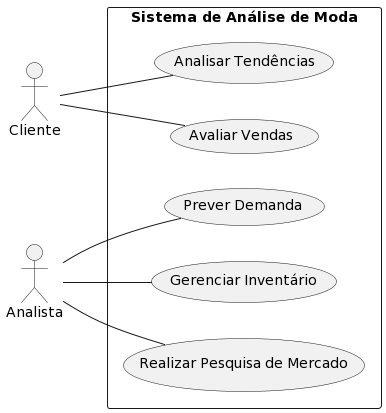
\includegraphics[width=0.9\textwidth]{imagens/casos-de-uso-diagrama.png}
    \caption{Diagrama de Casos de Uso para o Sistema de Moda Estatística}
\end{figure}

\subsection{Documentação dos Casos de Uso}
\begin{description}
    \item[Caso de Uso 1:] \textbf{Usuário Realiza Login} - O usuário insere credenciais para acessar o sistema.
    \item[Caso de Uso 2:] \textbf{Entrada de Dados Estatísticos} - O usuário insere ou carrega um conjunto de dados para análise.
    \item[Caso de Uso 3:] \textbf{Visualização de Resultados} - Exibição dos resultados estatísticos em gráficos interativos e tabelas.
\end{description}

\newpage
\section{Diagrama(s) de Classes do Sistema}

\begin{figure}[h]
    \centering
    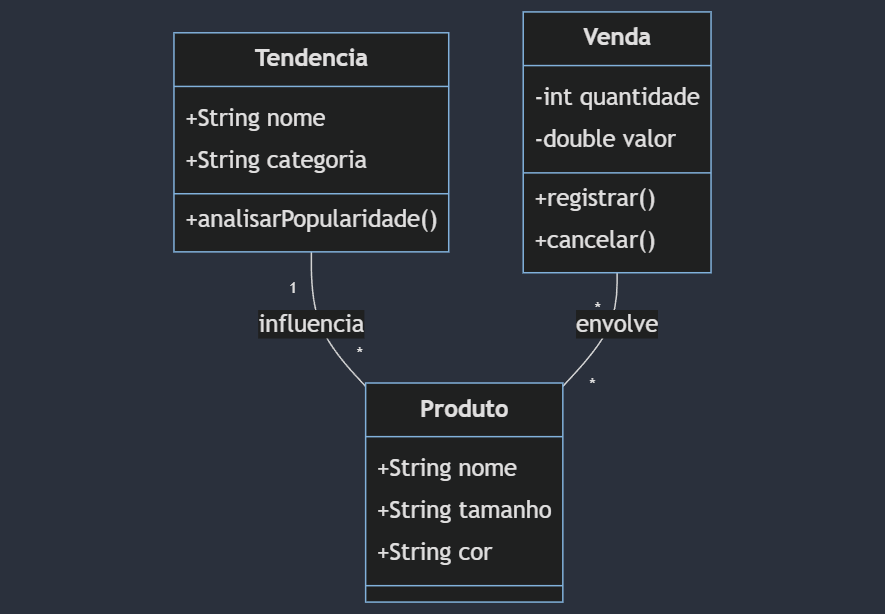
\includegraphics[width=0.9\textwidth]{imagens/classe-diagrama.png}
    \caption{Diagrama de Classes do Sistema de Moda Estatística}
\end{figure}

% Descreva as principais classes e suas relações aqui
\begin{description}
    \item[Classe Usuário:] Responsável pela gestão de informações do usuário.
    \item[Classe Dados:] Gerencia a entrada e armazenamento de dados estatísticos.
    \item[Classe Análise:] Realiza os cálculos estatísticos e determina a moda.
    \item[Classe Visualização:] Responsável pela criação de gráficos e tabelas.
\end{description}

\newpage
\section{Protótipos do Sistema}

\subsection{Protótipo da Interface de Usuário}
\begin{description}
    \item[Descrição:] A interface de usuário foi projetada para ser minimalista e intuitiva, com campos claros para entrada de dados e opções de visualização de resultados.
    \item[Implementação:] Utilização de HTML, CSS e JavaScript para interatividade.
\end{description}

\begin{figure}[h]
    \centering
    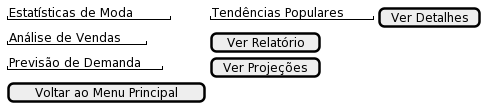
\includegraphics[width=0.9\textwidth]{imagens/prototipo-de-interface-usuario.png}
    \caption{Protótipo da Interface de Usuário}
\end{figure}

\section{Implementação dos Protótipos}

\subsection{Implementação do Protótipo de Interface de Usuário}
\begin{description}
    \item[Tecnologias Utilizadas:] HTML5, CSS3, JavaScript e frameworks como React para a construção da interface.
    \item[Funcionalidades:] Campos para entrada de dados, opções de visualização de resultados e suporte a múltiplos idiomas.
\end{description}

\subsection{Implementação do Protótipo de Análise de Dados}
\begin{description}
    \item[Tecnologias Utilizadas:] Python para cálculos estatísticos no back-end, com integração via APIs REST.
    \item[Funcionalidades:] Cálculo de moda, média, mediana e outras métricas estatísticas.
\end{description}

\end{document}
